\section{Requerimientos Funcionales}

\section{Requerimientos No Funcionales}

\section{Reglas de Negocio}

\section{Diagramas de Casos de Uso}
	En esta sección se presentan los casos de uso diseñados con base en los RF, RNF y RN. Están ordenados por módulos del sistema.
	\subsection{Módulo de autenticación}
	El módulo de autenticación tiene el siguiente caso de uso que permitirá al usuario autenticarse en la aplicación para poder hacer uso de ésta.
		\subsubsection{CU1: Iniciar sesión}
			\begin{figure}[htbp!]
				\centering
					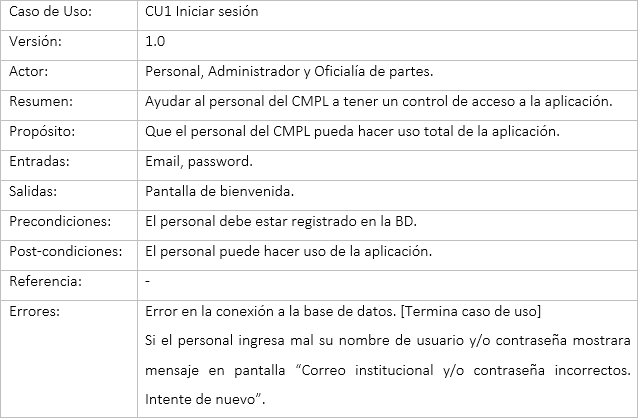
\includegraphics[width=0.8\textwidth]{images/CU/CU1}
					\caption{Caso de uso 1: Inicio de sesión.}
				\label{Tabla}
			\end{figure}
	\subsection{Módulo de Gestión de Usuarios}
	El módulo de Gestión de Usuarios poseé los siguientes casos de uso.
	
		\subsubsection{CU2: Dar de alta empleado del CMPL}
			\begin{figure}[htbp!]
				\centering
					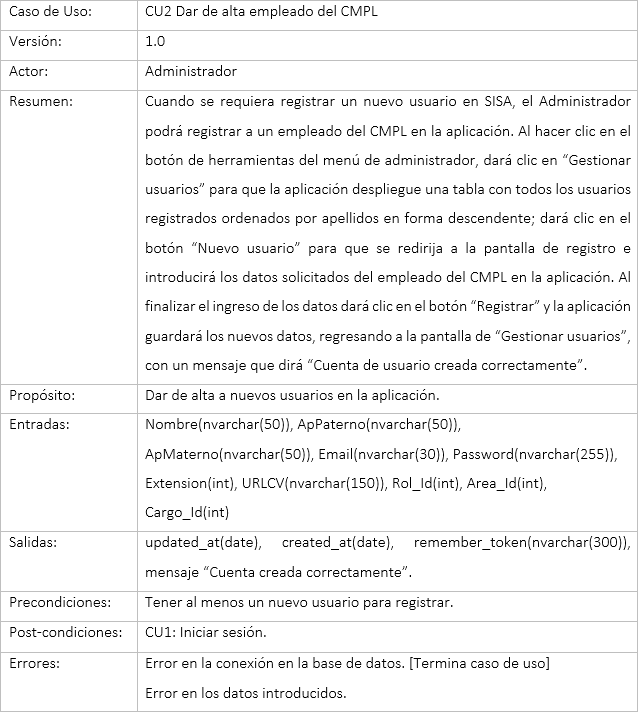
\includegraphics[width=0.8\textwidth]{images/CU/CU2}
					\caption{Caso de uso 2: Dar de alta empleado del CMPL.}
				\label{Tabla}
			\end{figure}
			
			\begin{itemize}
				\item Trayectoria principal:
					\begin{enumerate}
						\item El actor da clic en el menú de herramientas administrativas.
						\item La aplicación muestra el menú de herramientas administrativas.
						\item El actor da clic en la opción ``Gestionar usuarios''.
						\item La aplicación muestra la pantalla \IUref{IU32}, de gestión de usuarios.
						\item El actor da clic al botón ``Registrar nuevo usuario''.
						\item La aplicación muestra la pantalla \IUref{IU33}, de registro de usuarios.
						\item El actor ingresa los datos de usuario solicitados.
						\item El actor da clic al botón ``Registrar usuario''.
						\item La aplicación verifica si el correo electrónico, nombre, apellido paterno y apellido materno introducidos no han sido registrados anteriormente en una cuenta. \textsl{Trayectoria alternativa A}
						\item La aplicación registra en la base de datos los datos del nuevo usuario.
						\item La aplicación muestra la pantalla \IUref{IU32}, de gestión de usuarios, con el mensaje ``Cuenta de usuario creada correctamente''.
					\end{enumerate}
				\item Trayectorias alternativas:
					\begin{itemize}
						\item Trayectoria alternativa A: Si ya existe un registro con los datos introducidos.
							\begin{enumerate}
								\item La aplicación muestra la pantalla \IUref{IU33} con un mensaje que dice ``Error. Usuario registrado anteriormente''. Regresa al paso 7.
							\end{enumerate}
					\end{itemize}
			\end{itemize}
			
		\subsubsection{CU3: Modificar información de un empleado del CMPL}
			\begin{figure}[htbp!]
				\centering
					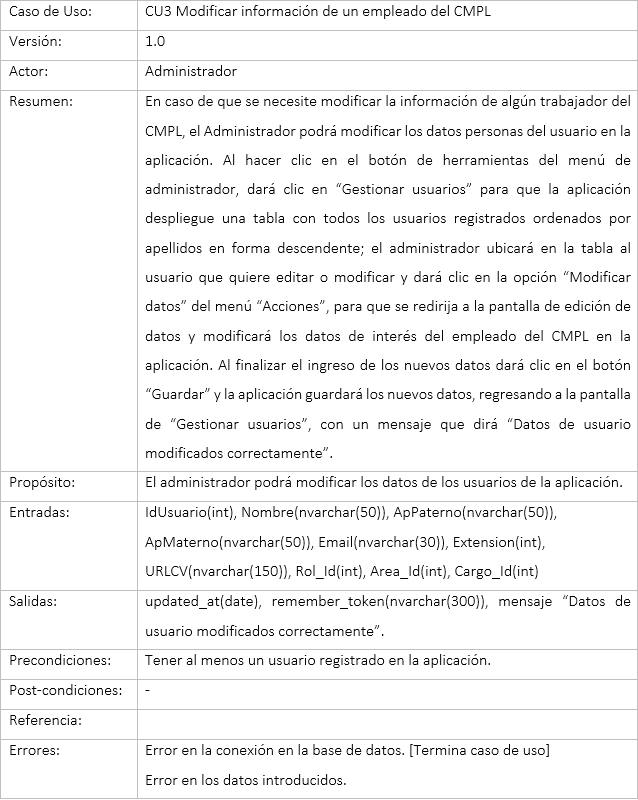
\includegraphics[width=0.8\textwidth]{images/CU/CU3}
					\caption{Caso de uso 3: Modificar información de un empleado del CMPL.}
				\label{Tabla}
			\end{figure}
			
			\begin{itemize}
				\item Trayectoria principal:
					\begin{enumerate}
						\item El actor da clic en el menú de herramientas administrativas.
						\item La aplicación muestra el menú de herramientas administrativas.
						\item El actor da clic en la opción ``Gestionar usuarios''.
						\item La aplicación muestra la pantalla \IUref{IU32}, de gestión de usuarios.
						\item El actor elije el usuario que desea editar y da clic al botón ``Acciones'' del menú de opciones de ese usuario.
						\item La aplicación muestra el menú de opciones del usuario seleccionado.
						\item El actor da clic en ``Editar usuario''.
						\item La aplicación muestra la pantalla \IUref{IU34}, de edición de usuarios.
						\item El actor cambia los datos de usuario deseados.
						\item El actor da clic al botón ``Guardar''.
						\item La aplicación verifica si el correo electrónico, nombre, apellido paterno y apellido materno introducidos no han sido registrados anteriormente en una cuenta. \textsl{Trayectoria alternativa A}
						\item La aplicación registra en la base de datos los nuevos datos del usuario seleccionado.
						\item La aplicación muestra la pantalla \IUref{IU32}, de gestión de usuarios, con el mensaje ``Datos de usuario modificados correctamente''.
					\end{enumerate}
				\item Trayectorias alternativas:
					\begin{itemize}
						\item Trayectoria alternativa A: Si ya existe un registro con los datos introducidos.
							\begin{enumerate}
								\item La aplicación muestra la pantalla \IUref{IU33} con un mensaje que dice ``Error. Usuario registrado anteriormente con los mismos datos''. Regresa al paso 9.
							\end{enumerate}
					\end{itemize}
			\end{itemize}
		
		\subsubsection{CU4: Desactivar cuenta de usuario}
			\begin{figure}[htbp!]
				\centering
					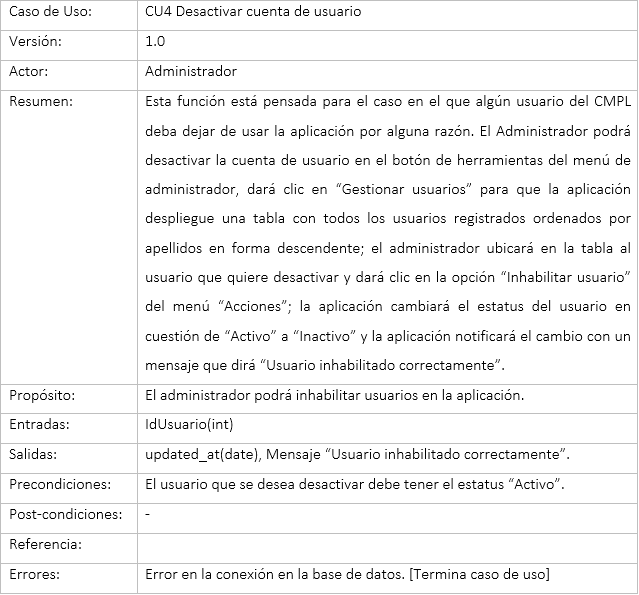
\includegraphics[width=0.8\textwidth]{images/CU/CU4}
					\caption{Caso de uso 4: Desactivar cuenta de usuario.}
				\label{Tabla}
			\end{figure}
			
			\begin{itemize}
				\item Trayectoria principal:
					\begin{enumerate}
						\item El actor da clic en el menú de herramientas administrativas.
						\item La aplicación muestra el menú de herramientas administrativas.
						\item El actor da clic en la opción ``Gestionar usuarios''.
						\item La aplicación muestra la pantalla \IUref{IU32}, de gestión de usuarios.
						\item El actor elije el usuario que desea editar y da clic al botón ``Acciones'' del menú de opciones de ese usuario.
						\item La aplicación muestra el menú de opciones del usuario seleccionado.
						\item El actor da clic en ``Inhabilitar usuario''.
						\item La aplicación cambia en la base de datos el estado de ``Activo'' a ``Inactivo'' de la cuenta de usuario seleccionada.
						\item La aplicación muestra la pantalla \IUref{IU32}, de gestión de usuarios, con el mensaje ``Usuario inhabilitado correctamente''.
					\end{enumerate}
			\end{itemize}
			
			
		\subsubsection{CU5: Activar cuenta de usuario}
			\begin{figure}[htbp!]
				\centering
					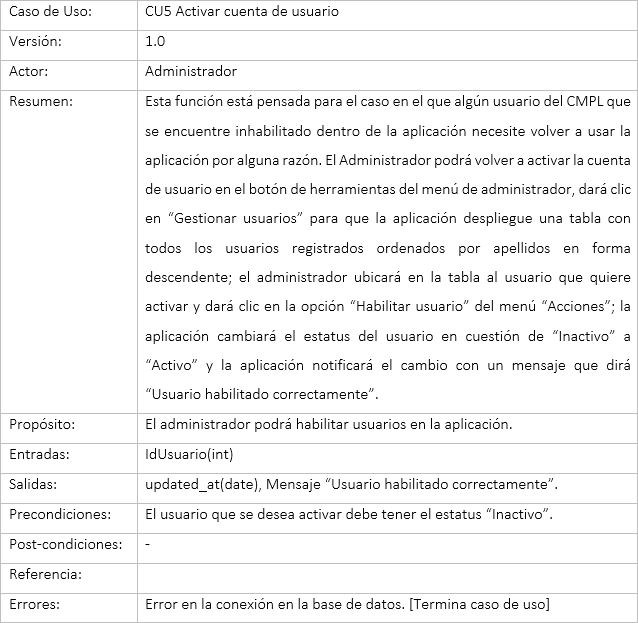
\includegraphics[width=0.8\textwidth]{images/CU/CU5}
					\caption{Caso de uso 5: Activar cuenta de usuario.}
				\label{Tabla}
			\end{figure}
			
			\begin{itemize}
				\item Trayectoria principal:
					\begin{enumerate}
						\item El actor da clic en el menú de herramientas administrativas.
						\item La aplicación muestra el menú de herramientas administrativas.
						\item El actor da clic en la opción ``Gestionar usuarios''.
						\item La aplicación muestra la pantalla \IUref{IU32}, de gestión de usuarios.
						\item El actor elije el usuario que desea editar y da clic al botón ``Acciones'' del menú de opciones de ese usuario.
						\item La aplicación muestra el menú de opciones del usuario seleccionado.
						\item El actor da clic en ``Habilitar usuario''.
						\item La aplicación cambia en la base de datos el estado de ``Inactivo'' a ``Activo'' de la cuenta de usuario seleccionada.
						\item La aplicación muestra la pantalla \IUref{IU32}, de gestión de usuarios, con el mensaje ``Usuario habilitado correctamente''.
					\end{enumerate}
			\end{itemize}
			
		\subsubsection{CU6: Ver directorio interno del CMPL}
			\begin{figure}[htbp!]
				\centering
					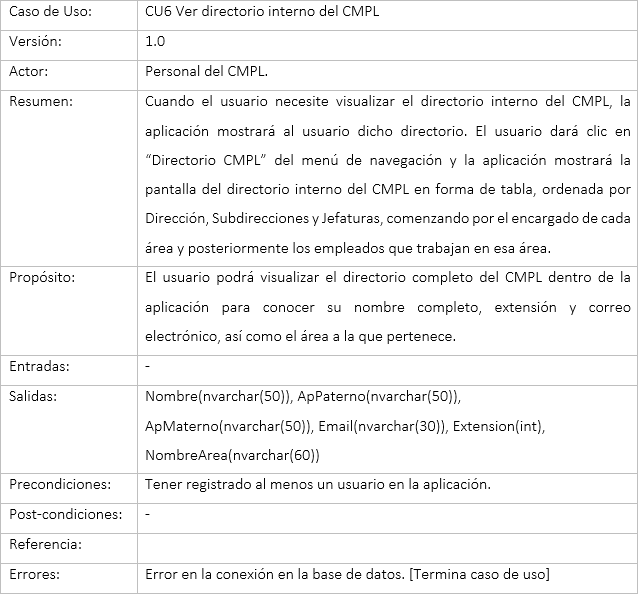
\includegraphics[width=0.8\textwidth]{images/CU/CU6}
					\caption{Caso de uso 6: Ver directorio interno del CMPL.}
				\label{Tabla}
			\end{figure}
			
			\begin{itemize}
				\item Trayectoria principal:
					\begin{enumerate}
						\item El actor va a la sección de Menú y da clic en ``Directorio CMPL''.
						\item La aplicación realiza la consulta a la base de datos y ordena los datos obtenidos por departamento o subdirección, incluyendo la Dirección.
						\item La aplicación muestra la pantalla \IUref{IU35}, del directorio interno del CMPL.
					\end{enumerate}
			\end{itemize}
			
		\subsubsection{CU7: Ver directorio interno del CMPL por área o departamento}
			\begin{figure}[htbp!]
				\centering
					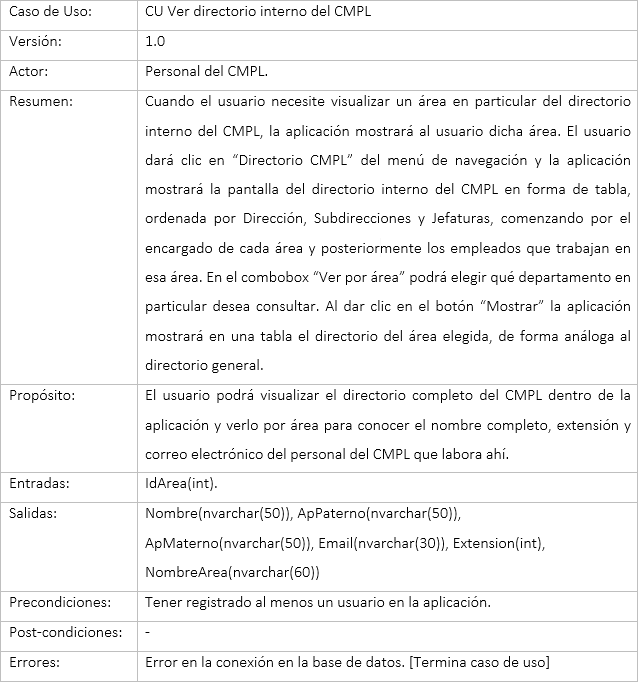
\includegraphics[width=0.8\textwidth]{images/CU/CU7}
					\caption{Caso de uso 7: Ver directorio interno del CMPL por área o departamento.}
				\label{Tabla}
			\end{figure}
			
			\begin{itemize}
				\item Trayectoria principal:
					\begin{enumerate}
						\item El actor va a la sección de Menú y da clic en ``Directorio CMPL''.
						\item La aplicación realiza la consulta a la base de datos y ordena los datos obtenidos por departamento o subdirección, incluyendo la Dirección.
						\item La aplicación muestra la pantalla \IUref{IU35}, del directorio interno del CMPL.
						\item El actor selecciona qué departamento desea ver únicamente en la opción ``Ver por área''.
						\item El actor da clic al botón ``Mostrar''.
						\item La aplicación muestra la pantalla \IUref{35}, con una tabla donde se muestra el listado de empleados y encargado del departamento seleccionado.
					\end{enumerate}
			\end{itemize}
			
		\subsubsection{CU8: Buscar empleado del CMPL por nombre}
			\begin{figure}[htbp!]
				\centering
					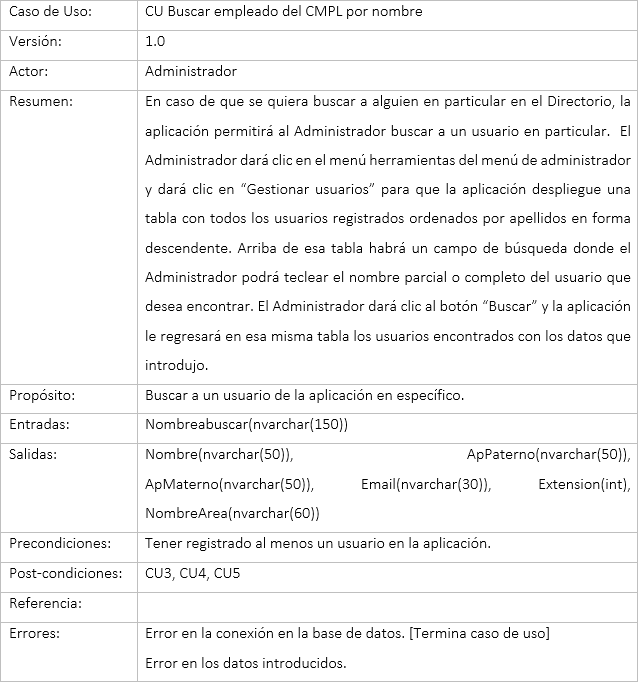
\includegraphics[width=0.8\textwidth]{images/CU/CU8}
					\caption{Caso de uso 8: Buscar empleado del CMPL por nombre.}
				\label{Tabla}
			\end{figure}
			
			\begin{itemize}
				\item Trayectoria principal:
					\begin{enumerate}
						\item El actor da clic en el menú de herramientas administrativas.
						\item La aplicación muestra el menú de herramientas administrativas.
						\item El actor da clic en la opción ``Gestionar usuarios''.
						\item La aplicación muestra la pantalla \IUref{IU32}, de gestión de usuarios.
						\item El actor introduce en el campo de texto el nombre parcial o completo del usuario que desea localizar y da clic al botón ``Buscar''. 
						\item La aplicación busca en la base de datos el nombre parcial o completo introducido en el campo de búsqueda. \textsl{Trayectoria alternativa A}
						\item La aplicación muestra nuevamente la pantalla \IUref{IU32} con los registros que coinciden en parte o totalmente con los datos ingresados en el campo de búsqueda.
					\end{enumerate}
				\item Trayectorias alternativas:
					\begin{itemize}
						\item Trayectoria alternativa A: Cuando no se encuentra coincidencia alguna en la base de datos con lo introducido en el campo de búsqueda.
							\begin{enumerate}
								\item La aplicación muestra la pantalla \IUref{32} con un mensaje de notificación que dice ``No se encontraron coincidencias con la información proporcionada''. Regresa al paso 5. 
							\end{enumerate}
					\end{itemize}
			\end{itemize}
			
		\subsubsection{CU9: Restablecer contraseña de usuario}
			\begin{figure}[htbp!]
				\centering
					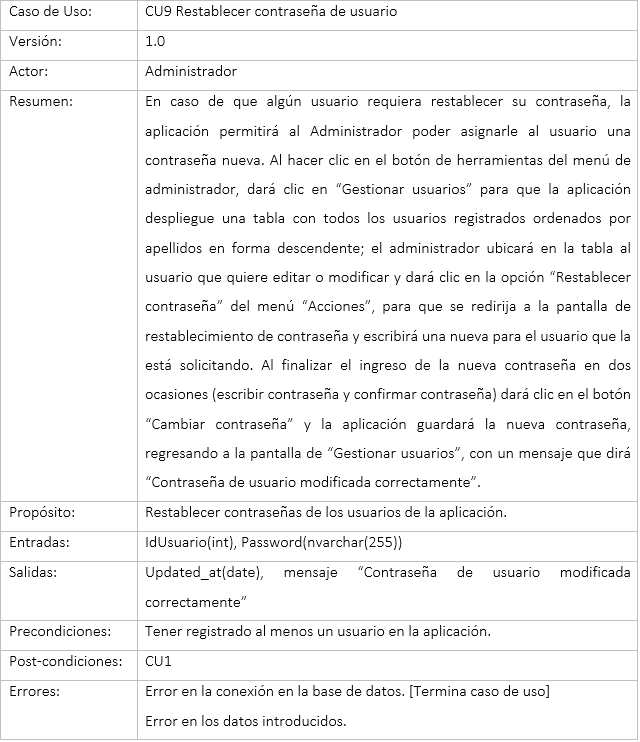
\includegraphics[width=0.8\textwidth]{images/CU/CU9}
					\caption{Caso de uso 9: Restablecer contraseña de usuario.}
				\label{Tabla}
			\end{figure}
			
			\begin{itemize}
				\item Trayectoria principal:
					\begin{enumerate}
						\item El actor da clic en el menú de herramientas administrativas.
						\item La aplicación muestra el menú de herramientas administrativas.
						\item El actor da clic en la opción ``Gestionar usuarios''.
						\item La aplicación muestra la pantalla \IUref{IU32}, de gestión de usuarios.
						\item El actor elije el usuario que desea editar y da clic al botón ``Acciones'' del menú de opciones de ese usuario.
						\item La aplicación muestra el menú de opciones del usuario seleccionado.
						\item El actor da clic en ``Restablecer contraseña''.
						\item La aplicación muestra la pantalla \IUref{IU36}, de restablecimiento de contraseña.
						\item El actor teclea una nueva contraseña.
						\item El actor vuelve a teclear la nueva contraseña.
						\item El actor da clic al botón ``Cambiar contraseña''.
						\item La aplicación verifica que ambos campos de contraseña coincidan. \textsl{Trayectoria alternativa A}
						\item La aplicación verifica que la contraseña no sea menor a 6 dígitos. \textsl{Trayectoria alternativa B}
						\item La aplicación cambia la contraseña del usuario seleccionado.
						\item La aplicación muestra la pantalla \IUref{IU32}, de gestión de usuarios, con el mensaje ``Contraseña de usuario modificada correctamente''.
					\end{enumerate}
				\item Trayectorias alternativas:
					\begin{itemize}
						\item Trayectoria alternativa A: Si los campos de contraseña no coinciden.
							\begin{enumerate}
								\item La aplicación muestra la pantalla \IUref{IU36}, con un mensaje de error diciendo ``Las contraseñas no coinciden. Por favor, ingrese de nuevo la nueva contraseña''. Regresa al paso 9.
							\end{enumerate}
						\item Trayectoria alternativa B: Si la longitud de la contraseña es menor a 6.
							\begin{enumerate}
								\item La aplicación muestra la pantalla \IUref{IU36}, con un mensaje de error diciendo ``La contraseña es menor a 6 dígitos. Por favor, teclee una contraseña con al menos 6 dígitos''. Regresa al paso 9.
							\end{enumerate}
					\end{itemize}
			\end{itemize}
			
		\subsubsection{CU10: Cambiar contraseña}
			\begin{figure}[htbp!]
				\centering
					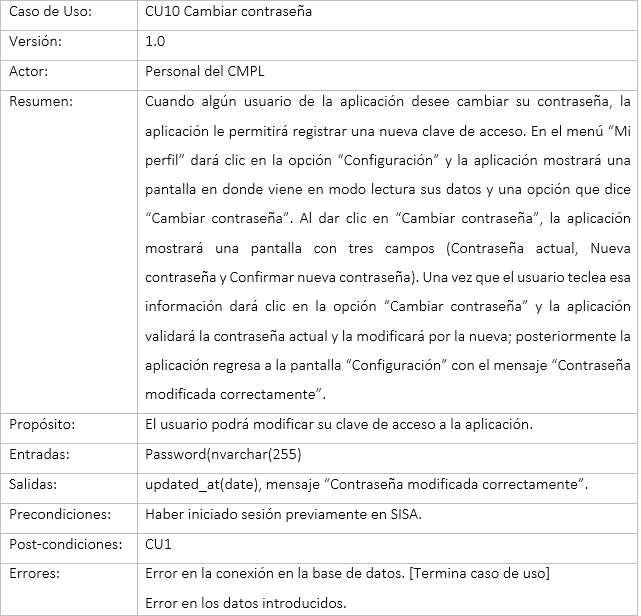
\includegraphics[width=0.8\textwidth]{images/CU/CU10}
					\caption{Caso de uso 10: Cambiar contraseña.}
				\label{Tabla}
			\end{figure}
			
			\begin{itemize}
				\item Trayectoria principal:
					\begin{enumerate}
						\item El actor da clic en el menú ``Mi perfil''.
						\item La aplicación muestra el menú del perfil de usuario.
						\item El actor da clic en la opción ``Configuración''.
						\item La aplicación muestra la pantalla \IUref{IU37}, de Mi perfil.
						\item El actor selecciona el botón ``Cambiar contraseña''.
						\item La aplicación muestra la pantalla \IUref{IU36}, de restablecimiento de contraseña.
						\item El actor teclea una nueva contraseña.
						\item El actor vuelve a teclear la nueva contraseña.
						\item El actor da clic al botón ``Cambiar contraseña''.
						\item La aplicación verifica que ambos campos de contraseña coincidan. \textsl{Trayectoria alternativa A}
						\item La aplicación verifica que la contraseña no sea menor a 6 dígitos. \textsl{Trayectoria alternativa B}
						\item La aplicación cambia la contraseña del usuario seleccionado.
						\item La aplicación muestra la pantalla \IUref{IU37}, de Mi perfil, con el mensaje ``Contraseña modificada correctamente''.
					\end{enumerate}
				\item Trayectorias alternativas:
					\begin{itemize}
						\item Trayectoria alternativa A: Si los campos de contraseña no coinciden.
							\begin{enumerate}
								\item La aplicación muestra la pantalla \IUref{IU36}, con un mensaje de error diciendo ``Las contraseñas no coinciden. Por favor, ingrese de nuevo la nueva contraseña''. Regresa al paso 8.
							\end{enumerate}
						\item Trayectoria alternativa B: Si la longitud de la contraseña es menor a 6.
							\begin{enumerate}
								\item La aplicación muestra la pantalla \IUref{IU36}, con un mensaje de error diciendo ``La contraseña es menor a 6 dígitos. Por favor, teclee una contraseña con al menos 6 dígitos''. Regresa al paso 8.
							\end{enumerate}
					\end{itemize}
			\end{itemize}
			
		\subsubsection{CU11: }
			\begin{figure}[htbp!]
				\centering
					%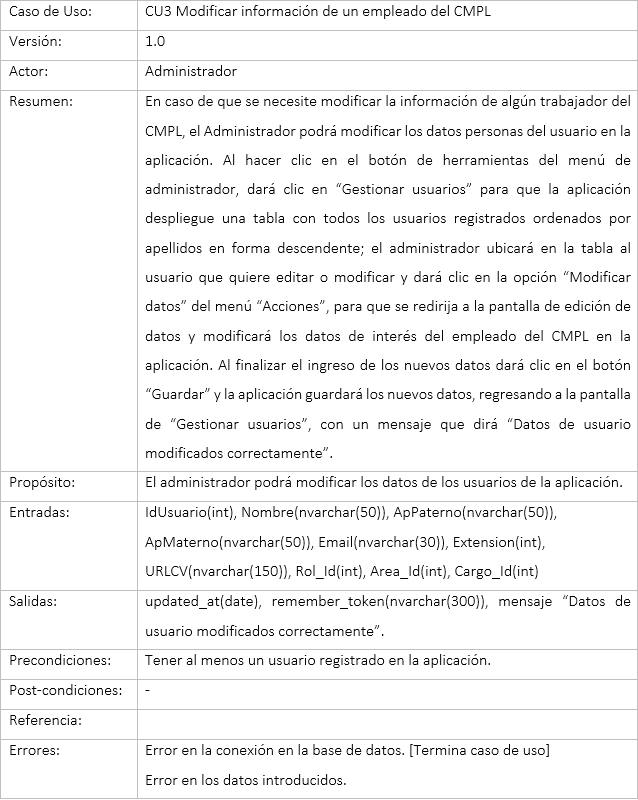
\includegraphics[width=0.8\textwidth]{images/CU/CU3}
					\caption{Caso de uso n: .}
				\label{Tabla}
			\end{figure}
			
			\begin{itemize}
				\item Trayectoria principal:
					\begin{enumerate}
						\item El actor va a la sección de correspondencia 
					\end{enumerate}
				\item Trayectorias alternativas:
					\begin{itemize}
						\item Trayectoria alternativa A:
							\begin{enumerate}
								\item La aplicación muestra un mensaje de error.
							\end{enumerate}
					\end{itemize}
			\end{itemize}

A continuación se muestran los casos de uso para los oficios salientes.
\begin{figure}[htbp!]
		\centering
			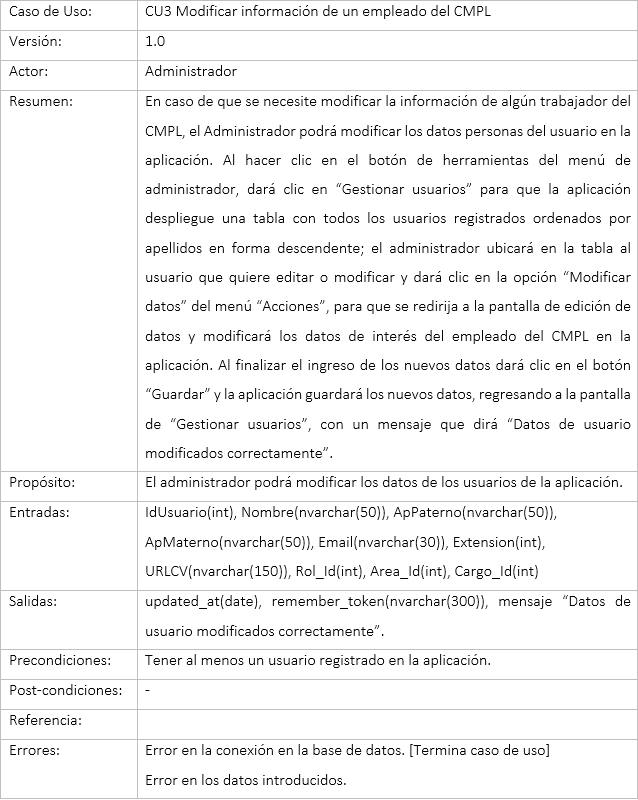
\includegraphics[width=0.8\textwidth]{images/CU/CU3}
		\caption{Caso de uso 3: Registrar oficio saliente.}
		\label{Tabla}
	\end{figure}

\begin{itemize}
	\item Trayectoria principal:
	\begin{enumerate}
		\item El actor va a la sección de correspondencia 
		\item La aplicación muestra la pantalla IU4 Correspondencia.
		\item El actor presiona el botón “Nuevo oficio”.
		\item La aplicación muestra la interfaz IU4.1 para el registro de oficios.
		\item El actor introduce los datos requeridos para el registro del oficio.
		\item El actor presiona el botón “Adjuntar documento”.
		\item CU27 Guardar Archivo.
		\item El usuario presiona el botón “Registrar”. 
		\item La aplicación hace la validación de los datos introducidos. \textsl{Trayectoria alternativa A} 
		\item La aplicación muestra el mensaje MSG2 de que el registro se realizó de forma exitosa.
		\item Fin del caso de uso.
	\end{enumerate}
	
	\item Trayectorias alternativas:
	\begin{itemize}
		\item Trayectoria alternativa A:
			\begin{enumerate}
				\item La aplicación muestra un mensaje de error.
				\item La aplicación resalta los campos en el formulario con errores.
				\item El usuario corrige los errores en el formulario.
				\item Continua en trayectoria del CU3 en paso 8.
			\end{enumerate}
	\end{itemize}
\end{itemize}

